\documentclass[11pt,a4paper]{article}

\usepackage[margin=2.2cm]{geometry}
\usepackage{graphicx}
\usepackage{xcolor}
\usepackage{hyperref}
\usepackage{booktabs}

\definecolor{wasla}{RGB}{2,132,199}
\hypersetup{
  colorlinks=true,
  linkcolor=wasla,
  urlcolor=wasla,
  pdftitle={Internship Report - Wasla Transport Analytics},
  pdfauthor={Yasmine Ghomrassi}
}

\setlength{\parindent}{0pt}
\setlength{\parskip}{7pt}

\begin{document}

% ------------------------------------------------------------------
\begin{titlepage}
  \centering
  \vspace*{0.8cm}
  
\includegraphics[width=0.42\textwidth]{bacekdendglitch_logo.png}\\[1.1cm]

  {\LARGE\bfseries Internship Report}\\[0.5cm]
  {\large\color{wasla}\bfseries Transport Analytics \& Operations Intelligence\\[2pt]
  for the Wasla Platform}\\[2.0cm]

  \begin{tabular}{ll}
    \textbf{Student}            & Yasmine Ghomrassi \\
    \textbf{Degree program}     & Master's Degree in Statistics and Data Science \\
    \textbf{University}         & University of Palermo (Italy) \\[0.4cm]
    \textbf{Host company}       & Backend Glitch Inc. (backendglitch.com) \\
    \textbf{Company supervisor} & Mr.\ Samer Gassouma (CEO) \\[0.4cm]
    \textbf{Location}           & Monastir, Tunisia \\
    \textbf{Period}             & 1 July 2026 to 25 September 2026 \\
  \end{tabular}

  \vfill
  \begin{minipage}[t]{0.45\textwidth}
    \centering
    \textbf{Company supervisor}\\[0.6cm]
    
\includegraphics[width=3.8cm]{stamp_e-sign.png}\\[0.25cm]
    {\small Mr.\ Samer Gassouma\\ CEO, Backend Glitch Inc.}
  \end{minipage}
  \hfill
  \begin{minipage}[t]{0.45\textwidth}
    \centering
    \textbf{University coordinator}\\[1.9cm]
    \rule{0.9\textwidth}{0.4pt}\\[0.25cm]
    {\small Prof.\ Erasmo Vassallo\\ University of Palermo}
  \end{minipage}

  \vfill
  
\includegraphics[width=3.1cm]{qr_repo.png}\hspace{1.2cm}%
  
\includegraphics[width=3.1cm]{qr_platform.png}\\[0.25cm]
  {\small Project repository \hspace{3.2cm} Live platform}
\end{titlepage}

% ------------------------------------------------------------------
\section{Host institution}

Backend Glitch Inc.\ (\url{https://backendglitch.com}) is a software company based in
Monastir, Tunisia. The company builds software solutions for companies and for the
clients who come to it: it works mainly on fintech and crypto solutions and on
backend solutions, and it also develops its own products, some of which are still on
the way. One of these projects is
\emph{Wasla}, a transport management platform that the company built as a solution
for its client \textbf{Dhraief Service de Transport} (\url{https://www.dhraief.live/}),
the operator of the Monastir Centre and Jammel Monastir stations.

\begin{center}
  
\includegraphics[width=0.22\textwidth]{dhraief_logo.png}\\[2pt]
  {\small Dhraief Service de Transport, the client behind the Wasla platform}
\end{center}

Wasla is in production at both stations, with a third station (Ksar Hlel) planned.
On a normal day the platform handles everything that happens at a station: passenger
bookings, vehicle dispatching, day passes, route scheduling, ticket printing and
staff shift tracking. The fleet counts 113 vehicles of eight seats each, serving five
destinations. The system has been collecting data since April 2026, and by the time I
joined there was more than a year's worth of bookings, trips and sales sitting in the
databases with nobody looking at it analytically. That was the whole point of my
internship.

\section{Dates and location}

I did my internship in Monastir, Tunisia, from 1 July 2026 to 25 September 2026,
working in person at the company under the supervision of Mr.\ Samer Gassouma, the
CEO. Most of my time was spent in the office and on the station servers, which are
only reachable from inside the local network.

\section{Objectives of the approved project}

The training plan agreed with the university listed six objectives:

\begin{enumerate}
  \item Understand the architecture and operational workflow of the Wasla platform.
  \item Analyse booking data, revenue streams and fleet utilisation statistically.
  \item Develop time-series models to forecast passenger volume.
  \item Design anomaly detection for booking patterns.
  \item Build analytical dashboards for operations monitoring and KPIs.
  \item Deploy the analytical services in a cloud environment (Docker, Linux VPS).
\end{enumerate}

\section{Work actually performed}

The work naturally fell into five phases, and this is roughly how my three months
went.

\subsection*{Phase 1: getting the data out}

The first thing I learned is that real production data does not wait for you in a CSV
file. The two stations each run their own PostgreSQL database on their own server,
accessible only over SSH tunnels, and for good reasons I was given read-only access.
I wrote an extraction pipeline that pulls eight tables per station (bookings, trips,
day passes, routes, vehicles, staff, print jobs and staff transactions) into parquet
files, then a cleaning layer that merges the two stations into one dataset. This was
more delicate than it sounds: the two databases do not even agree on column names
(seats are \texttt{booked\_seats} in one and \texttt{seats\_booked} in the other),
and each station uses its own destination IDs. I built a mapping between the two
namespaces so the five routes become comparable across stations. In the end the
cleaned dataset holds \textbf{1,582,729 bookings} from October 2025 to October 2026,
plus 15,470 trips and 39,792 day passes.

Two discoveries from this phase shaped everything that followed. First, roughly 93\%
of the bookings in the system are \emph{ghost bookings}: pre-generated drafts that
were never actually sold. Only about 6.6\% are verified tickets. Second, the word
``revenue'' means two different things in this business. What passengers pay
(\texttt{total\_amount}, which includes the driver's base fare) is one number; what
the station actually keeps (0.15 TND per seat plus 2 TND per day pass) is another,
about fourteen times smaller. I decided from the start that every chart, table and
KPI would say explicitly which revenue it is showing, because mixing the two makes
the numbers look wrong even when they are both right.

\subsection*{A closer look: how the data went from database to chart}

Since the pipeline is the part of my work I was asked about the most, here it is step
by step, with the actual commands I used every morning.

\textbf{Step 1. Open the tunnels.} Each station server is reached through a local
port forward, so the databases stay private while my scripts see them as local
Postgres instances.

\begin{verbatim}
ssh -fN -L 15432:localhost:5432 server@100.72.205.59
ssh -fN -L 15433:localhost:5432 ste@100.123.86.114
\end{verbatim}

\textbf{Step 2. Extract.} One script per station pulls every table and stores it as
parquet, batching large tables by id so a million-row bookings table never fills the
memory.

\begin{verbatim}
cd Phase_1/scripts
python3 01_extract.py jemmal
python3 01_extract.py monastir
\end{verbatim}

\textbf{Step 3. Clean and enrich.} A cleaning script unifies the two schemas, then a
features script adds the time variables (hour, weekday, month) and the real versus
ghost flag that every downstream analysis relies on.

\begin{verbatim}
cd .. && python3 02_clean.py && python3 03_features.py
\end{verbatim}

\textbf{Step 4. Plot and analyse.} The Phase 2 scripts group the enriched bookings
by hour, by day, by route and by vehicle and write both the numbers and the charts.
For example, the hourly flow chart below is exactly what came out of this step for
the whole history, and it is where the two peaks became visible.

\begin{figure}[h]
  \centering
  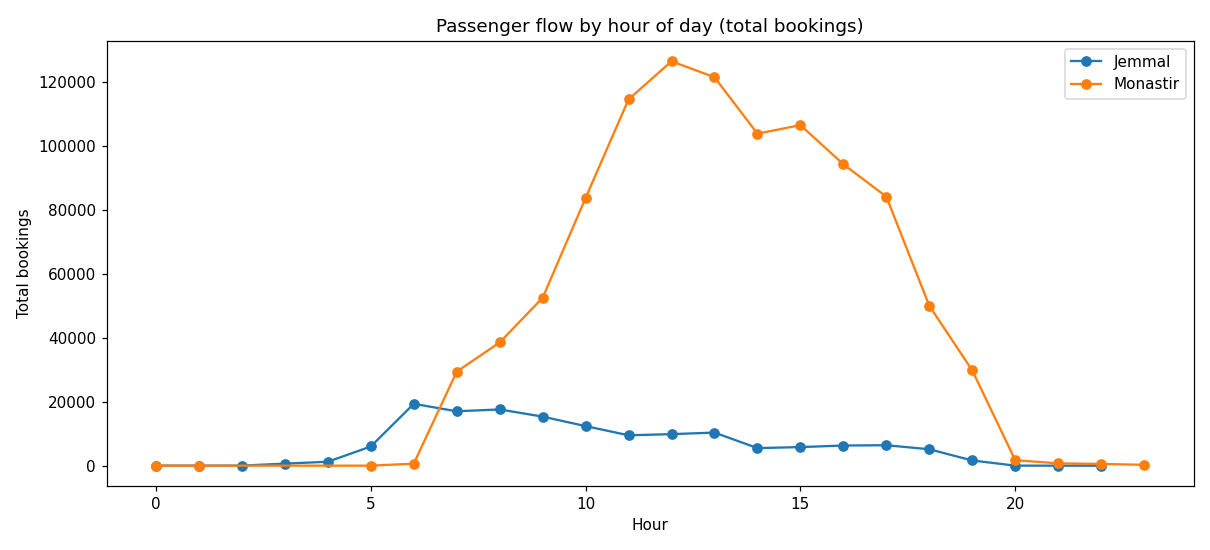
\includegraphics[width=0.8\textwidth]{../Phase_2/charts/flow_hourly.png}
  \caption{Passenger flow by hour of day, both stations. Jemmal peaks at 07h and
  Monastir at 12h.}
\end{figure}

\textbf{Step 5. Forecast and detect anomalies.} Phase 3 turns the daily series into
training data, runs the walk-forward cross-validation, refits the winning model on
the full series and produces the seven-day forecast with its confidence bands, then
scores every day with the three anomaly detectors.

\begin{figure}[h]
  \centering
  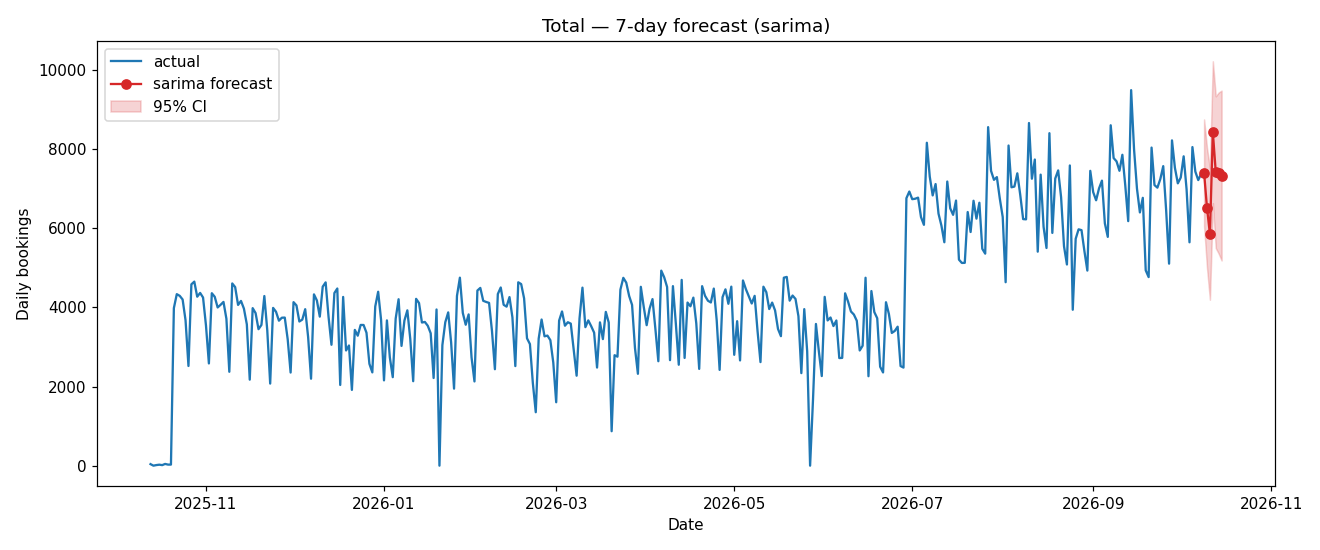
\includegraphics[width=0.8\textwidth]{../Phase_3/charts/forecast_total.png}
  \caption{Consolidated forecast: the SARIMA model with its walk-forward validation
  and the seven-day horizon ahead of the last training day.}
\end{figure}

\textbf{Step 6. Serve.} The dashboard reads these same artifacts, so whatever the
screen shows can always be traced back to a file, and the API exposes the same
numbers over HTTP with a live feed on top.

\subsection*{Phase 2: statistics}

With the data in shape I analysed passenger flow, revenue, routes and fleet use. The
clearest results: Jemmal peaks at 07h and Monastir at 12h (both around three times
their off-peak level), and Jemmal's fleet runs at a 90.9\% average load factor over
80 trips per vehicle. On the revenue side, the consolidated picture is
3,427,079 TND passenger-paid against 237,729 TND of station fees. The route table
showed something the operators already suspected: the Jemmal to Tunis line is the
premium route, with an average ticket of 15.85 TND and almost no ghost bookings,
while most other routes are dominated by drafts.

\subsection*{Phase 3: forecasting and anomaly detection}

I built daily demand series per station and for the network, then tested six
forecasting models: naive, seasonal naive, seasonal median, weekly mean, SARIMA and
Prophet. Instead of a single train/test split I used walk-forward
cross-validation, which feels like the only honest way to evaluate models on a time
series: the model always predicts the week after everything it has seen. Prophet
lost on every series; the winners were the simplest ones. Seasonal naive won for
Monastir (MAPE 8.5\%), naive won for Jemmal (6.3\%), and SARIMA won for the
consolidated total (6.0\%). For anomaly detection I combined three detectors, a
rolling z-score, a week over week difference z-score, and an Isolation Forest, and
flagged a day when at least two of them agree. This combination caught things a
single detector missed, like the two zero-booking days at Monastir that a plain
z-score would never see.

\subsection*{Phases 4 and 5: the dashboard, the API and the deployment}

The last stretch of the internship was software work. I built a seven-view analytics
dashboard (overview, passenger flow, revenue, routes, fleet, forecast, anomalies)
with Next.js and Recharts, designed so that every number on screen can be traced
back to the exact file that produced it. Behind it sits a small FastAPI service that
serves the analysis results and pushes a live minute-by-minute feed of today's
bookings over a WebSocket. Both are packaged with Docker. The dashboard is deployed
on Vercel at \url{https://wasla-analytics.vercel.app} (in static-data mode, since the
station databases live behind the local network), and the whole codebase, including
the data, is on GitHub at \url{https://github.com/yasmine-ghomrassi/wasla_Analytics}.

I also fixed my share of bugs along the way, the kind you only meet in production: a
partial extraction day that skewed the MAPE to absurd values, a WebSocket handshake
that FastAPI silently rejected because of a missing type annotation, and a
half-terabyte CSV that would not fit on GitHub until it was compressed. Each one
taught me something about verifying before trusting.

\begin{figure}[h]
  \centering
  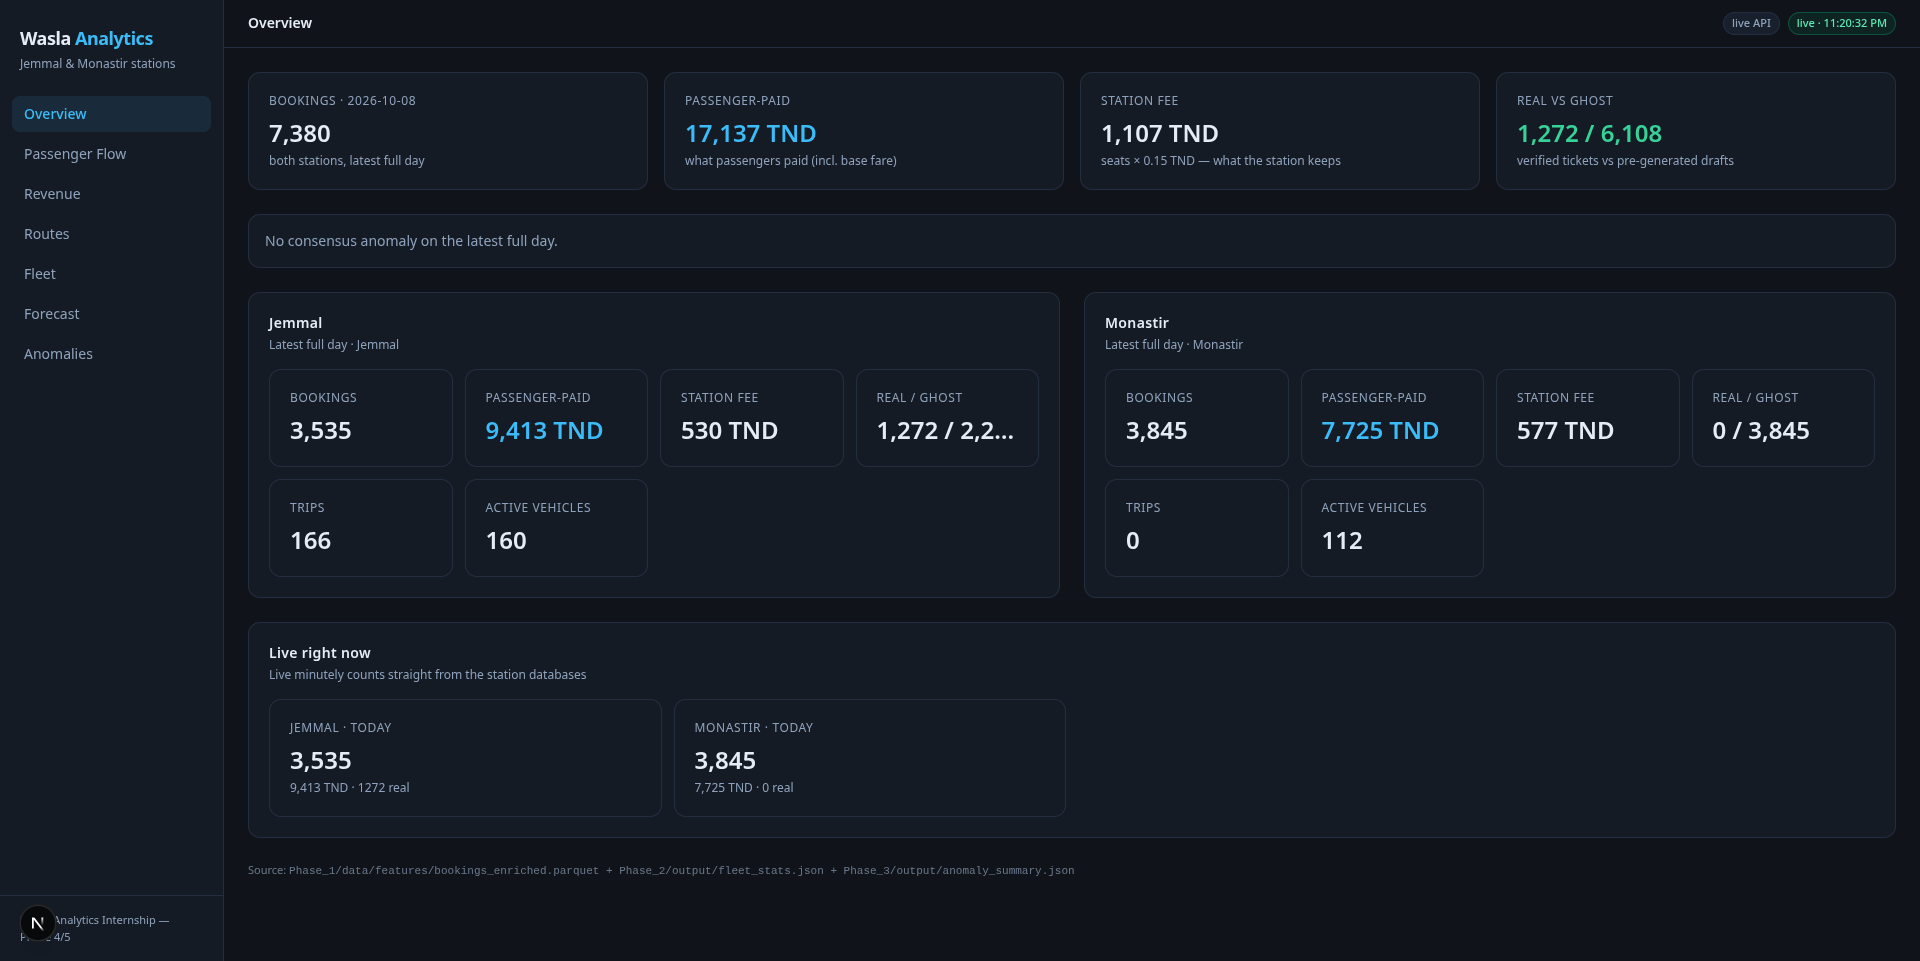
\includegraphics[width=0.85\textwidth]{../analytics_dashboard/docs/screenshots/1-overview.png}
  \caption{The Overview view of the dashboard, showing both revenue definitions and
  the live feed from the two stations.}
\end{figure}

\begin{figure}[h]
  \centering
  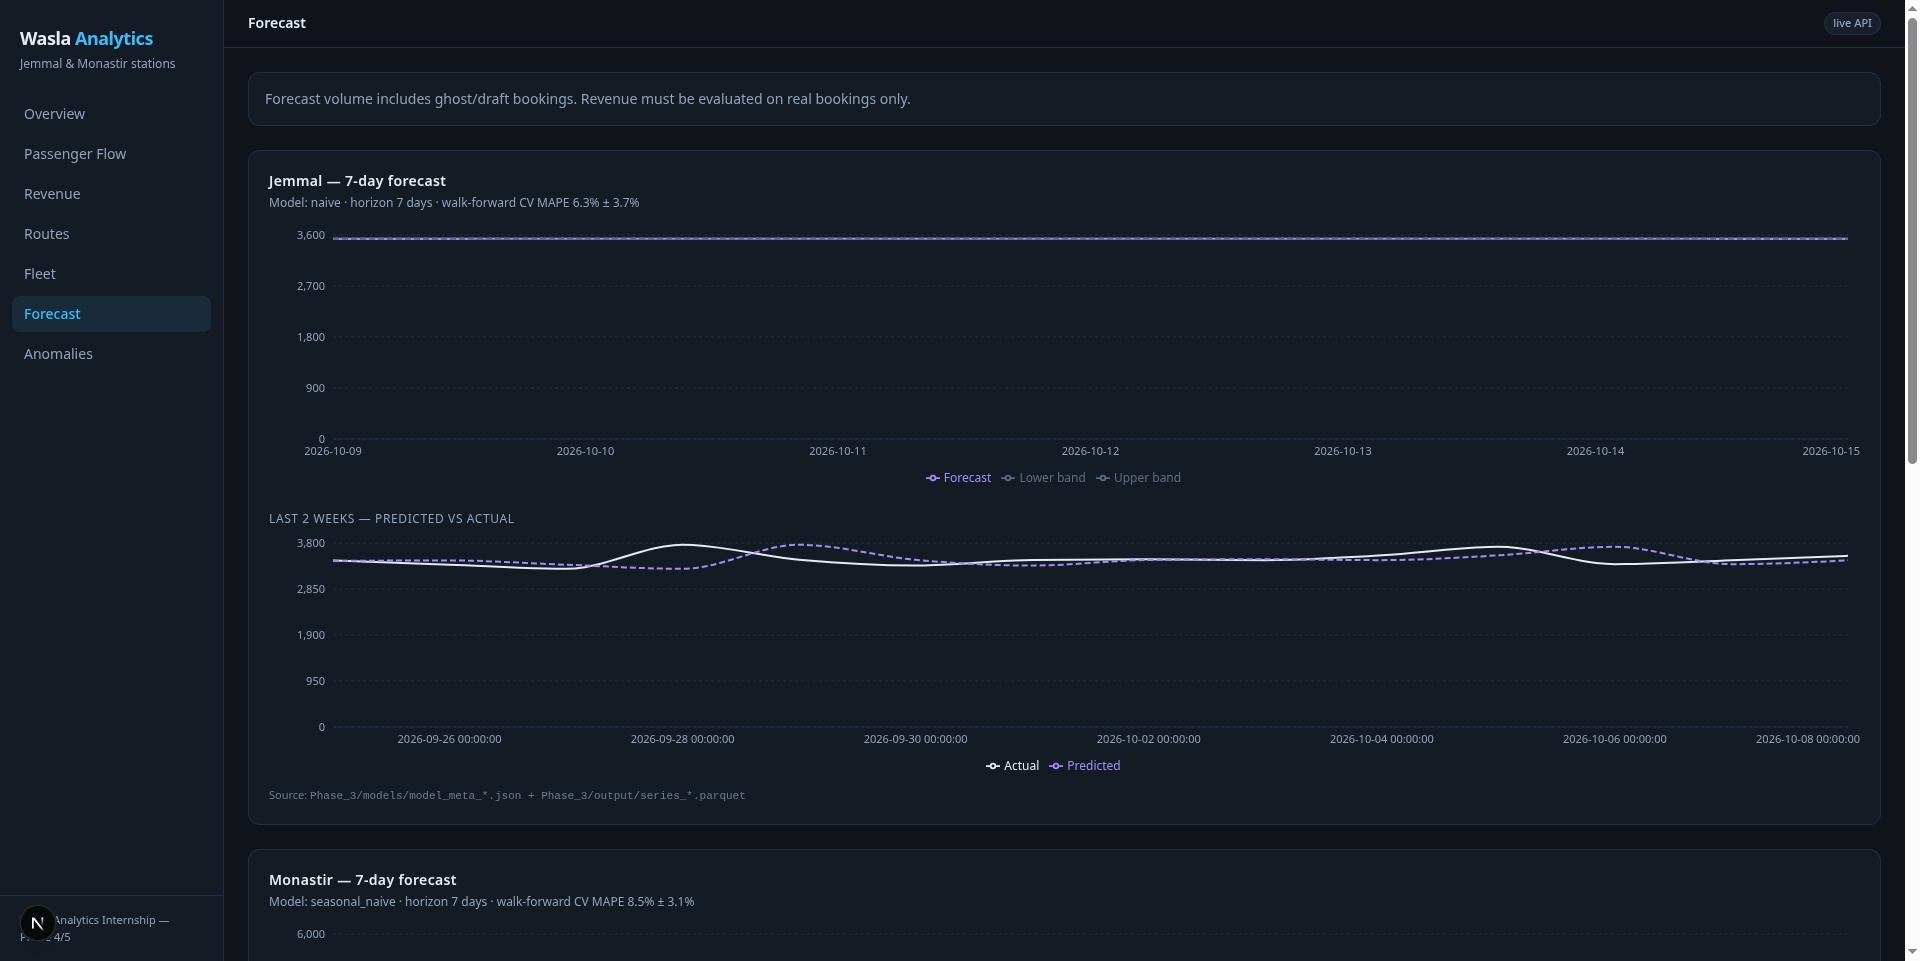
\includegraphics[width=0.85\textwidth]{../analytics_dashboard/docs/screenshots/6-forecast.png}
  \caption{Forecast view: seven-day forecasts with confidence bands and the
  cross-validation MAPE for each model.}
\end{figure}

\section{Technologies and methods used}

On the data side I worked with PostgreSQL over SSH tunnels, pandas and pyarrow for
processing, and parquet for storage. The statistical work used scipy and statsmodels
(descriptive analysis, time-of-day and weekday profiles, load factors), and the
machine-learning side used scikit-learn together with statsmodels for SARIMA and
Prophet. Model evaluation was always walk-forward cross-validation with MAPE and
RMSE, reported with their standard deviations across folds. The software side was
Next.js with TypeScript, Tailwind and Recharts for the dashboard, FastAPI with
WebSockets for the API, Docker and docker compose for packaging, and Git/GitHub with
Vercel for deployment. One habit I kept for the whole internship: whenever a number
looked surprising, I recomputed it from the raw parquet before touching any code.
More than once the bug was upstream.

\section{Results and outcomes}

In numbers: the pipeline now produces a clean, unified dataset of 1.58 million
bookings; the statistical reports quantify the two peaks (07h at Jemmal, 12h at
Monastir), the two revenue definitions (3.43M TND passenger-paid versus 238k TND
station fees), the five-route performance table and a 90.9\% fleet load factor; the
forecasting models deliver seven-day predictions with a cross-validated MAPE between
6.0\% and 8.5\%, served with confidence bands; and the anomaly system flagged a
booking spike at Jemmal on 29 June 2026 and two zero-booking days at Monastir. All of
it is visible in the dashboard, through the API, and reproducible from the GitHub
repository. For the company, the most actionable outcomes are probably the ghost
booking reality (revenue decisions should be made on verified tickets only) and the
morning peak, which leaves almost no slack in the fleet.

\section{How it relates to my Master's studies}

My degree in Statistics and Data Science at the University of Palermo prepared me for
a large part of this work, and the internship returned the favour by making all of it
concrete. The cross-validated model selection I used for the forecasts comes straight
from the time-series courses, but applying it to data where one station only has
four months of history, and where a single partial day can send the MAPE to 3000\%,
is a different experience from the textbook datasets. The anomaly detection work
(multiple detectors, consensus voting, handling zero-inflated series) is applied
statistical learning in the truest sense. And the deployment part, containers, a
REST API, a WebSocket feed, a public deployment, matches the cloud-computing
component of the programme. What the courses could not teach, the company did:
working with read-only production access, respecting a live system, and verifying
every result against its source before presenting it.

\section{Conclusion}

Looking back at the three months, the internship turned out to be a full pipeline
from database to dashboard, and I am glad it did: nothing less would have taught me
how every stage depends on the one before it. I learned to deal with messy,
inconsistent, real-world data; I built forecasting and anomaly-detection systems that
survived cross-validation rather than just fitting; and I shipped software that
people at the stations can actually open. The two findings that matter most for the
company, the ghost-booking reality and the dual revenue definitions, are now
measured, labelled and monitored instead of hidden in the database. I finished the
internship with a much clearer idea of what it means to do data science on a live
system, and I am grateful to Mr.\ Gassouma and the whole team for the opportunity.

\end{document}
